\documentclass{article}
\usepackage{mainPoly}

\title{Fonctions exponentielles}
\author{Terminale STMG2}
\date{}

\begin{document}
\maketitle
\section{Définition de l'exponentielle de base $a$}
\begin{tcolorbox}
On représente ci-contre les valeurs de la suite géométrique $(u_n)_{n \in \N}$ définie par $u_n = a^n$, avec $a > 0$.
\end{tcolorbox}
\begin{center}
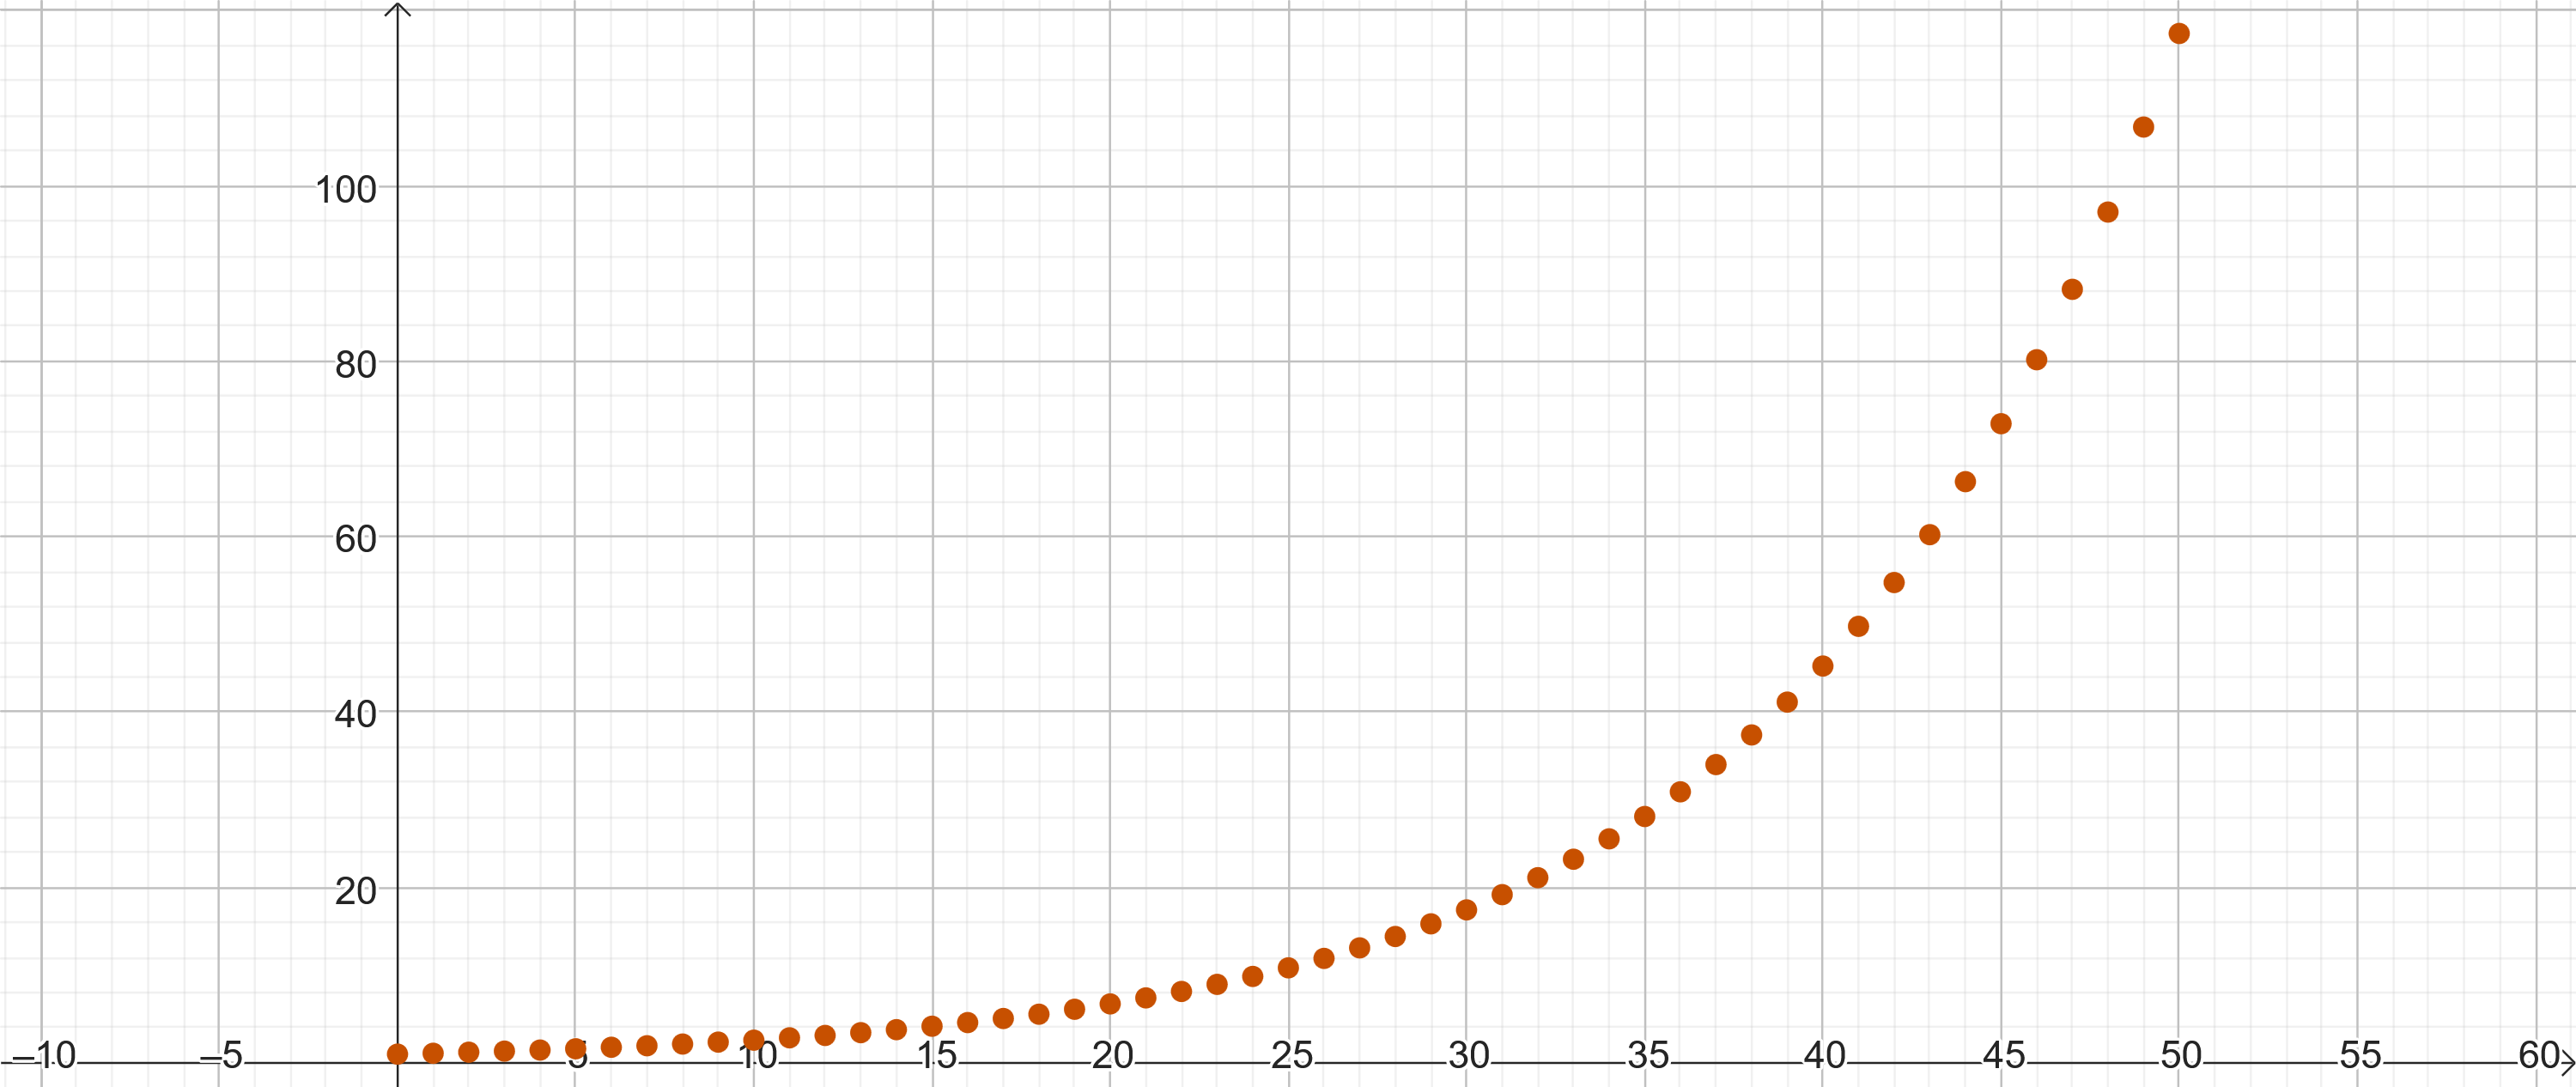
\includegraphics[width=\textwidth]{Suite_geometrique.png}
\end{center}
\begin{tcolorbox}
\begin{definition}
Le prolongement aux réels de la suite $u_n$ est appelée \textbf{fonction exponentielle de base $a$}. Pour tout $x$ réel, l'image de $x$ par cette fonction est notée $a^x$. En particulier, si $x < 0$, alors cette image est définie par:
\begin{equation*}
a^x = \dfrac{1}{a^{-x}}
\end{equation*}
\end{definition}    
\end{tcolorbox}
\begin{example}
À l'aide d'une calculatrice, donner la valeur des image de fonctions exponentielles suivantes :
\begin{enumquestions}
\item $2^{3,5} = $\answersline
\item $10,2^{0,2} = $\answersline
\item $0,6^{-5,4} = $\answersline
\end{enumquestions}
\end{example}
\newpage
\section{Représentation graphique}
On représente ci-dessous la courbe représentative d'une fonction exponentielle de base $a$. Elle correspond au prolongement des points de coordonnées $(n;a^n)$.
\vspace*{0.5cm}
\begin{center}
\begin{minipage}{0.45\textwidth}
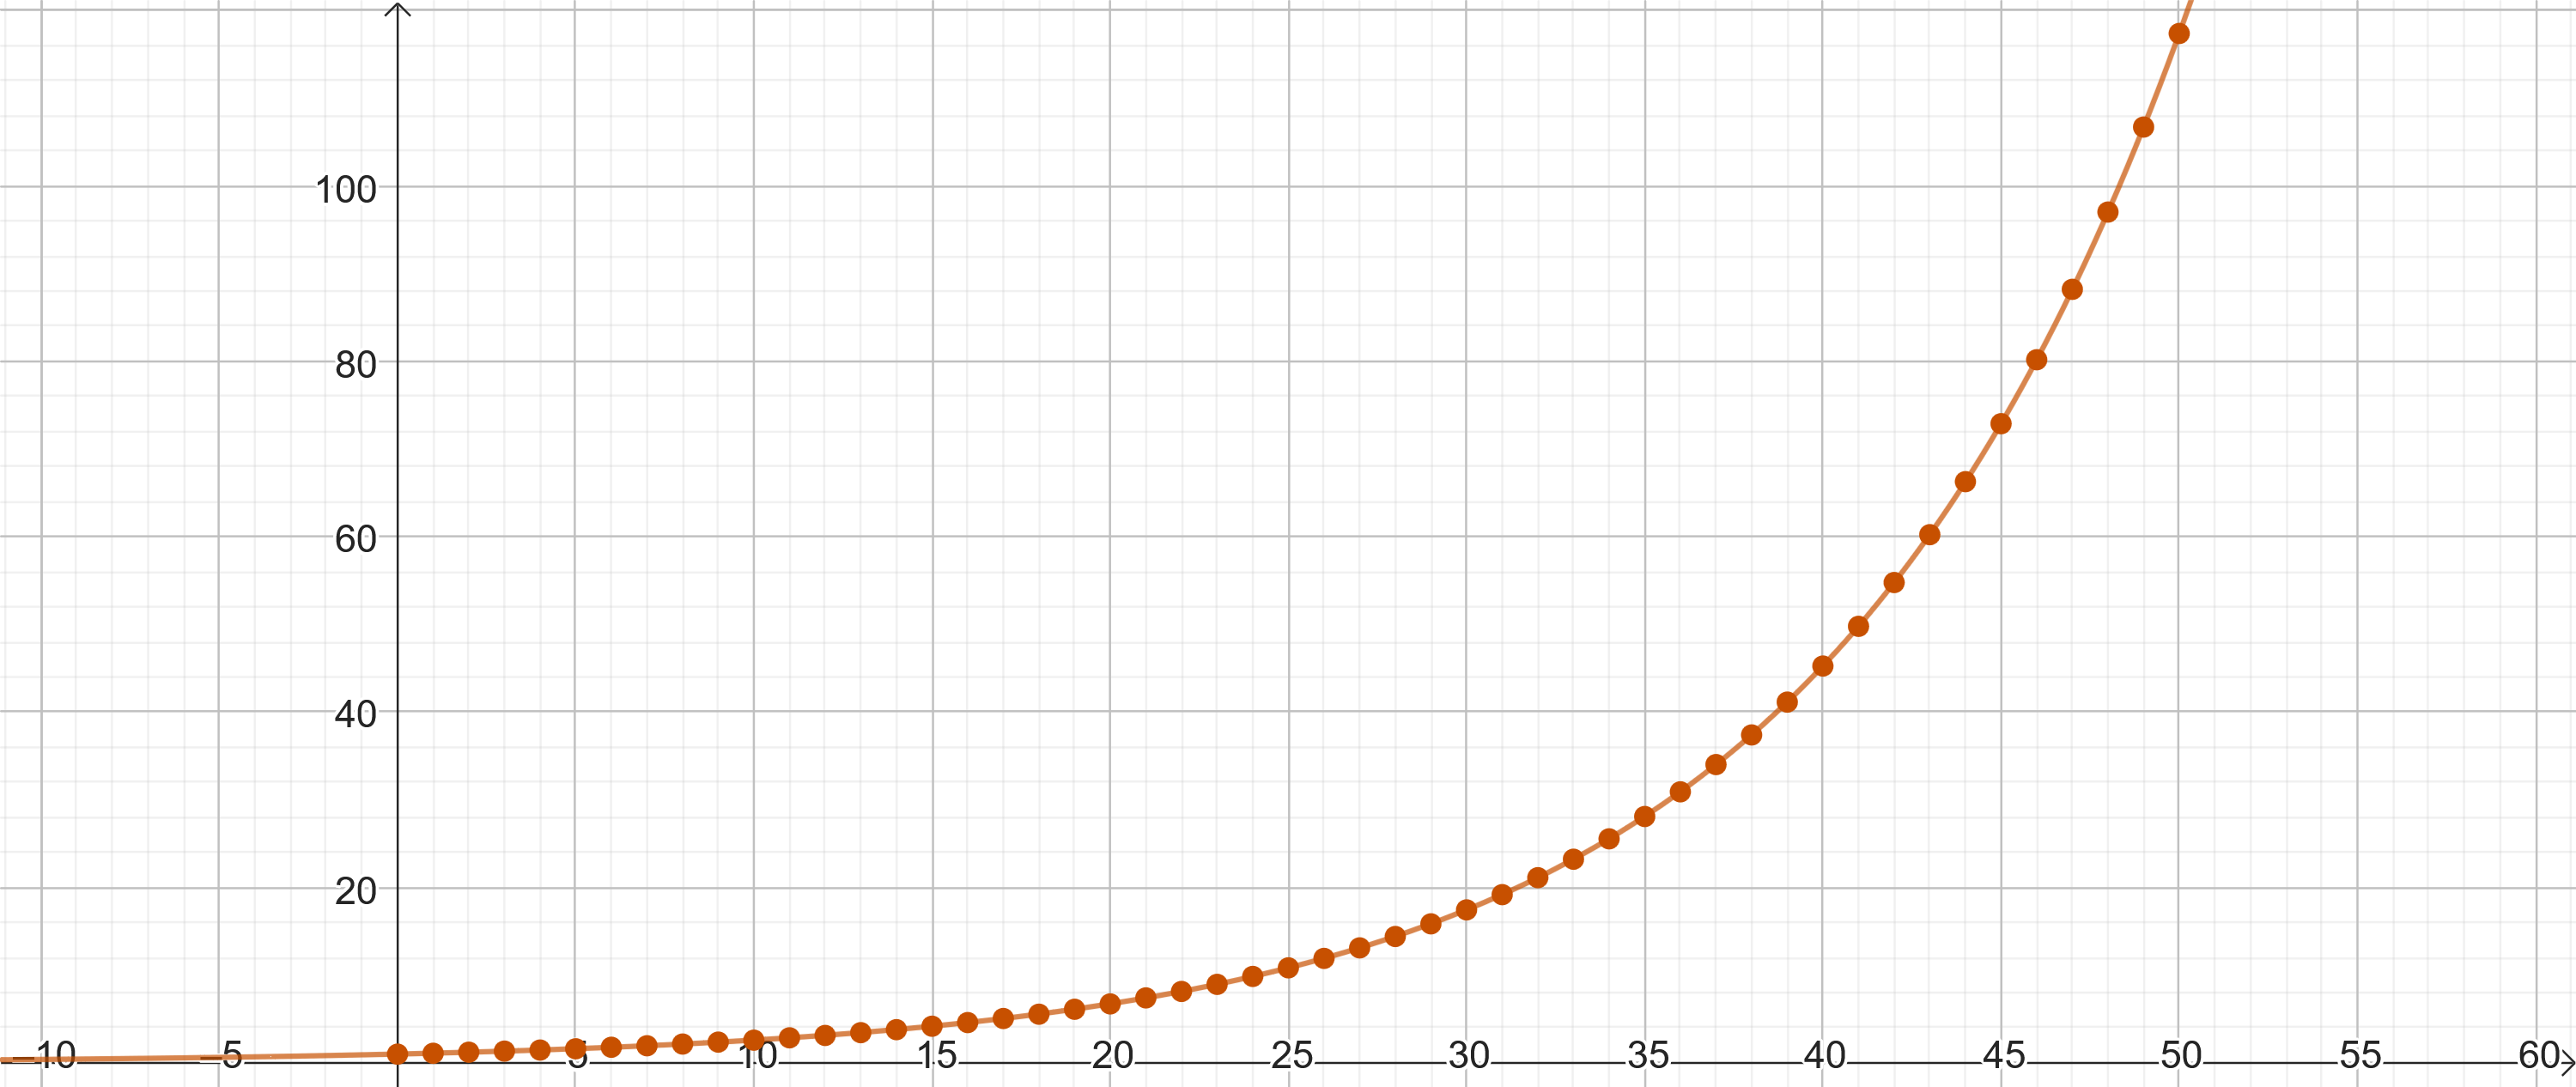
\includegraphics[width=\textwidth]{Fonction_exponentielle.png}
\end{minipage}
\begin{minipage}{0.45\textwidth}
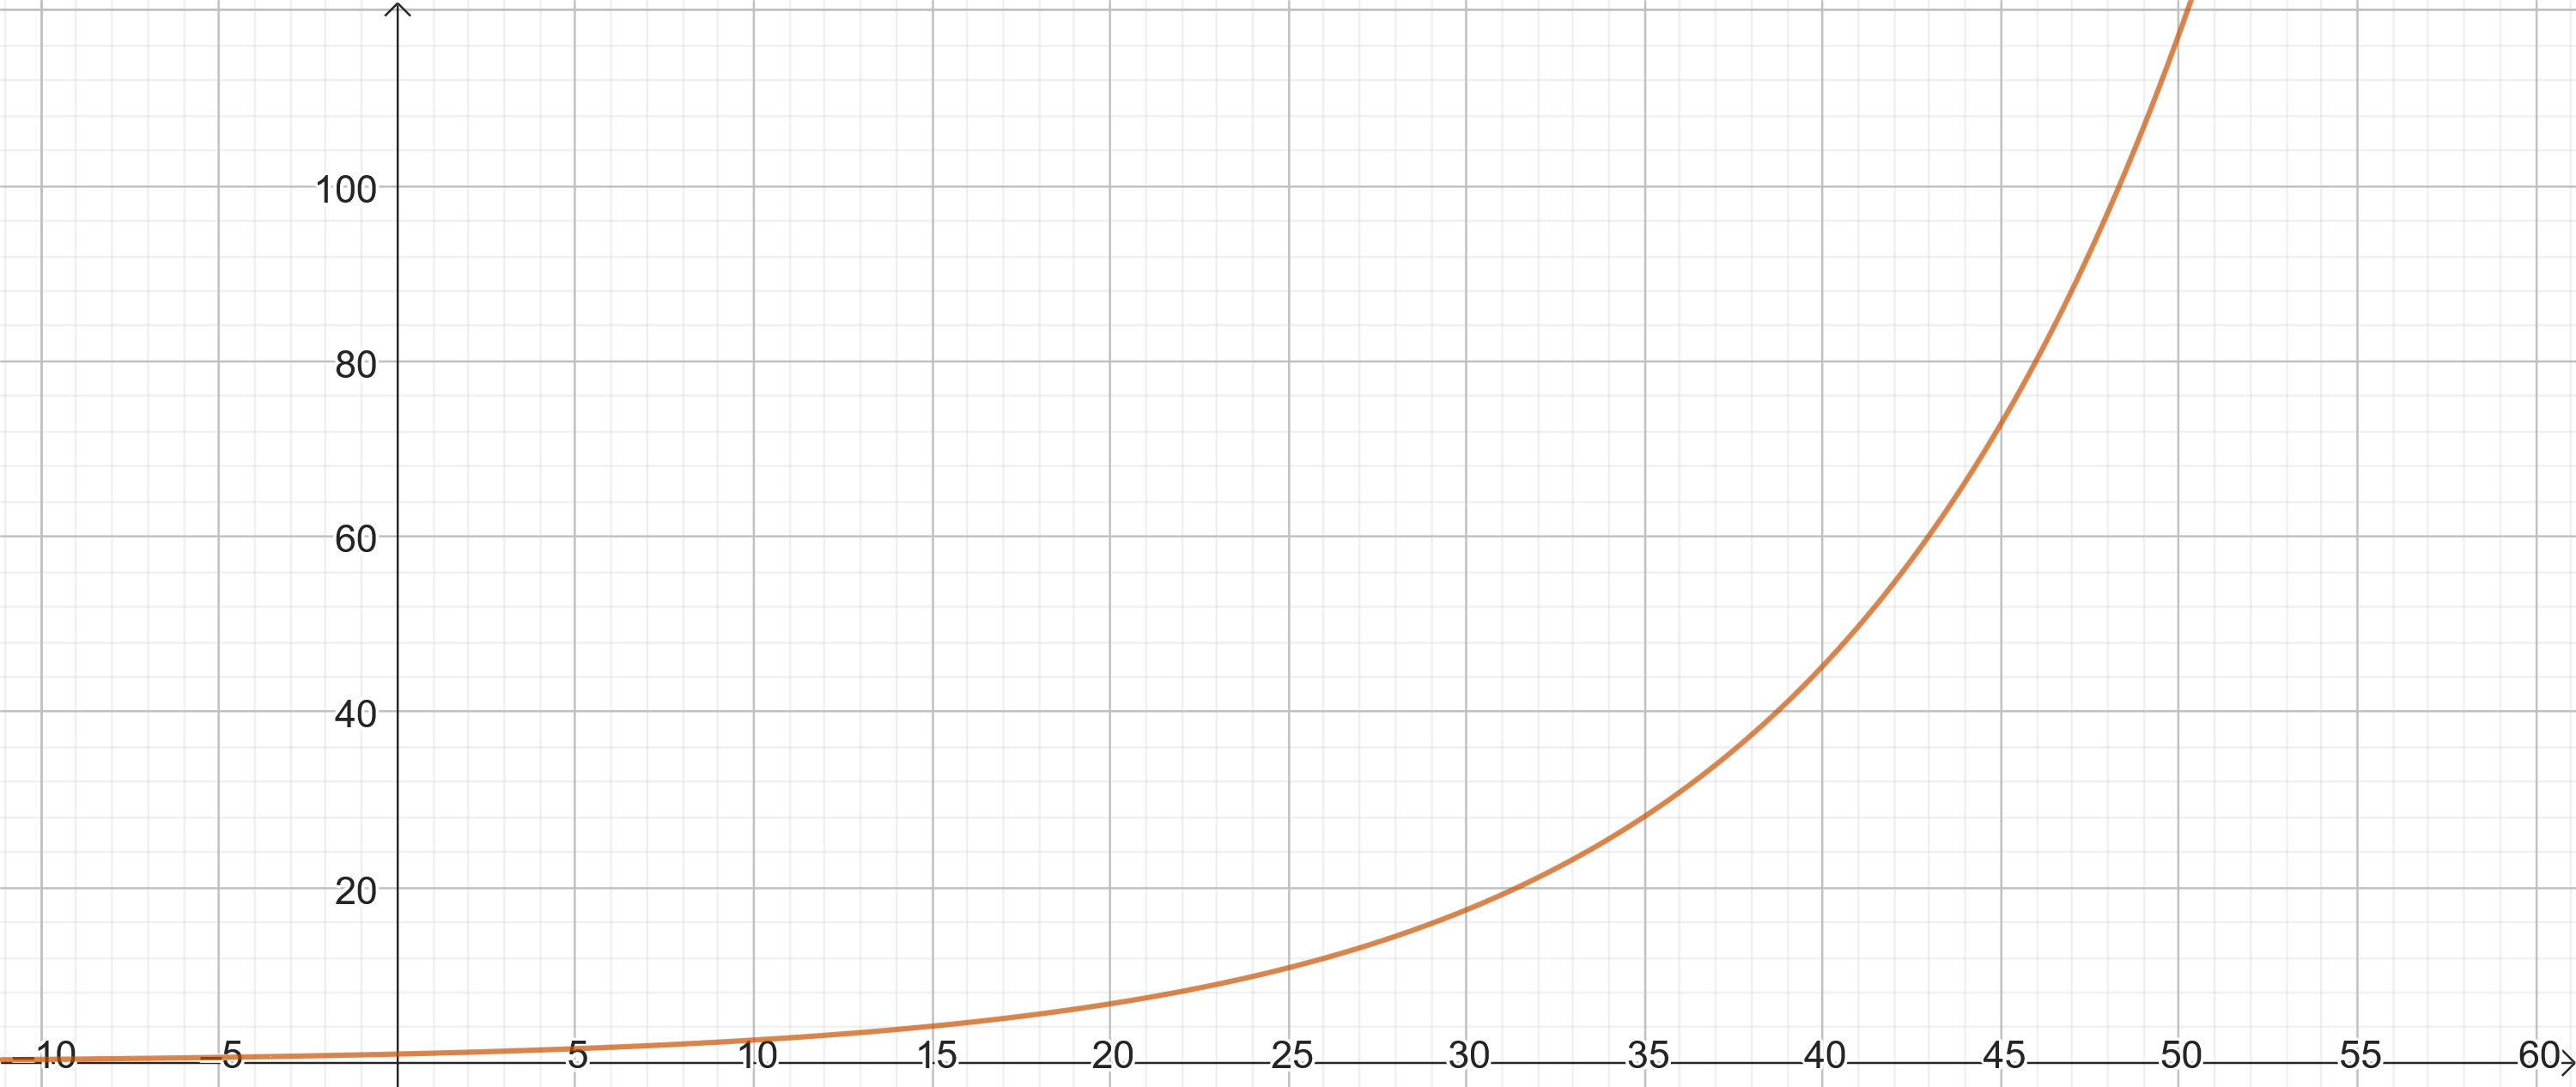
\includegraphics[width=\textwidth]{Fonction_exponentielle_2.png}
\end{minipage}
\end{center}
\section{Sens de variation}
\begin{tcolorbox}
\begin{proposition}
Soit $a > 0$ un nombre réel. Alors,
\begin{itemize}
\item La fonction exponentielle de base $a$ est strictement croissante si et seulement si $a > 1$. 
\item La fonction exponentielle de base $a$ est strictement décroissante si et seulement si $a < 1$. 
\item La fonction exponentielle de base $a$ est constante si et seulement si $a = 1$. 
\end{itemize}
\end{proposition}
\end{tcolorbox}
\begin{center}
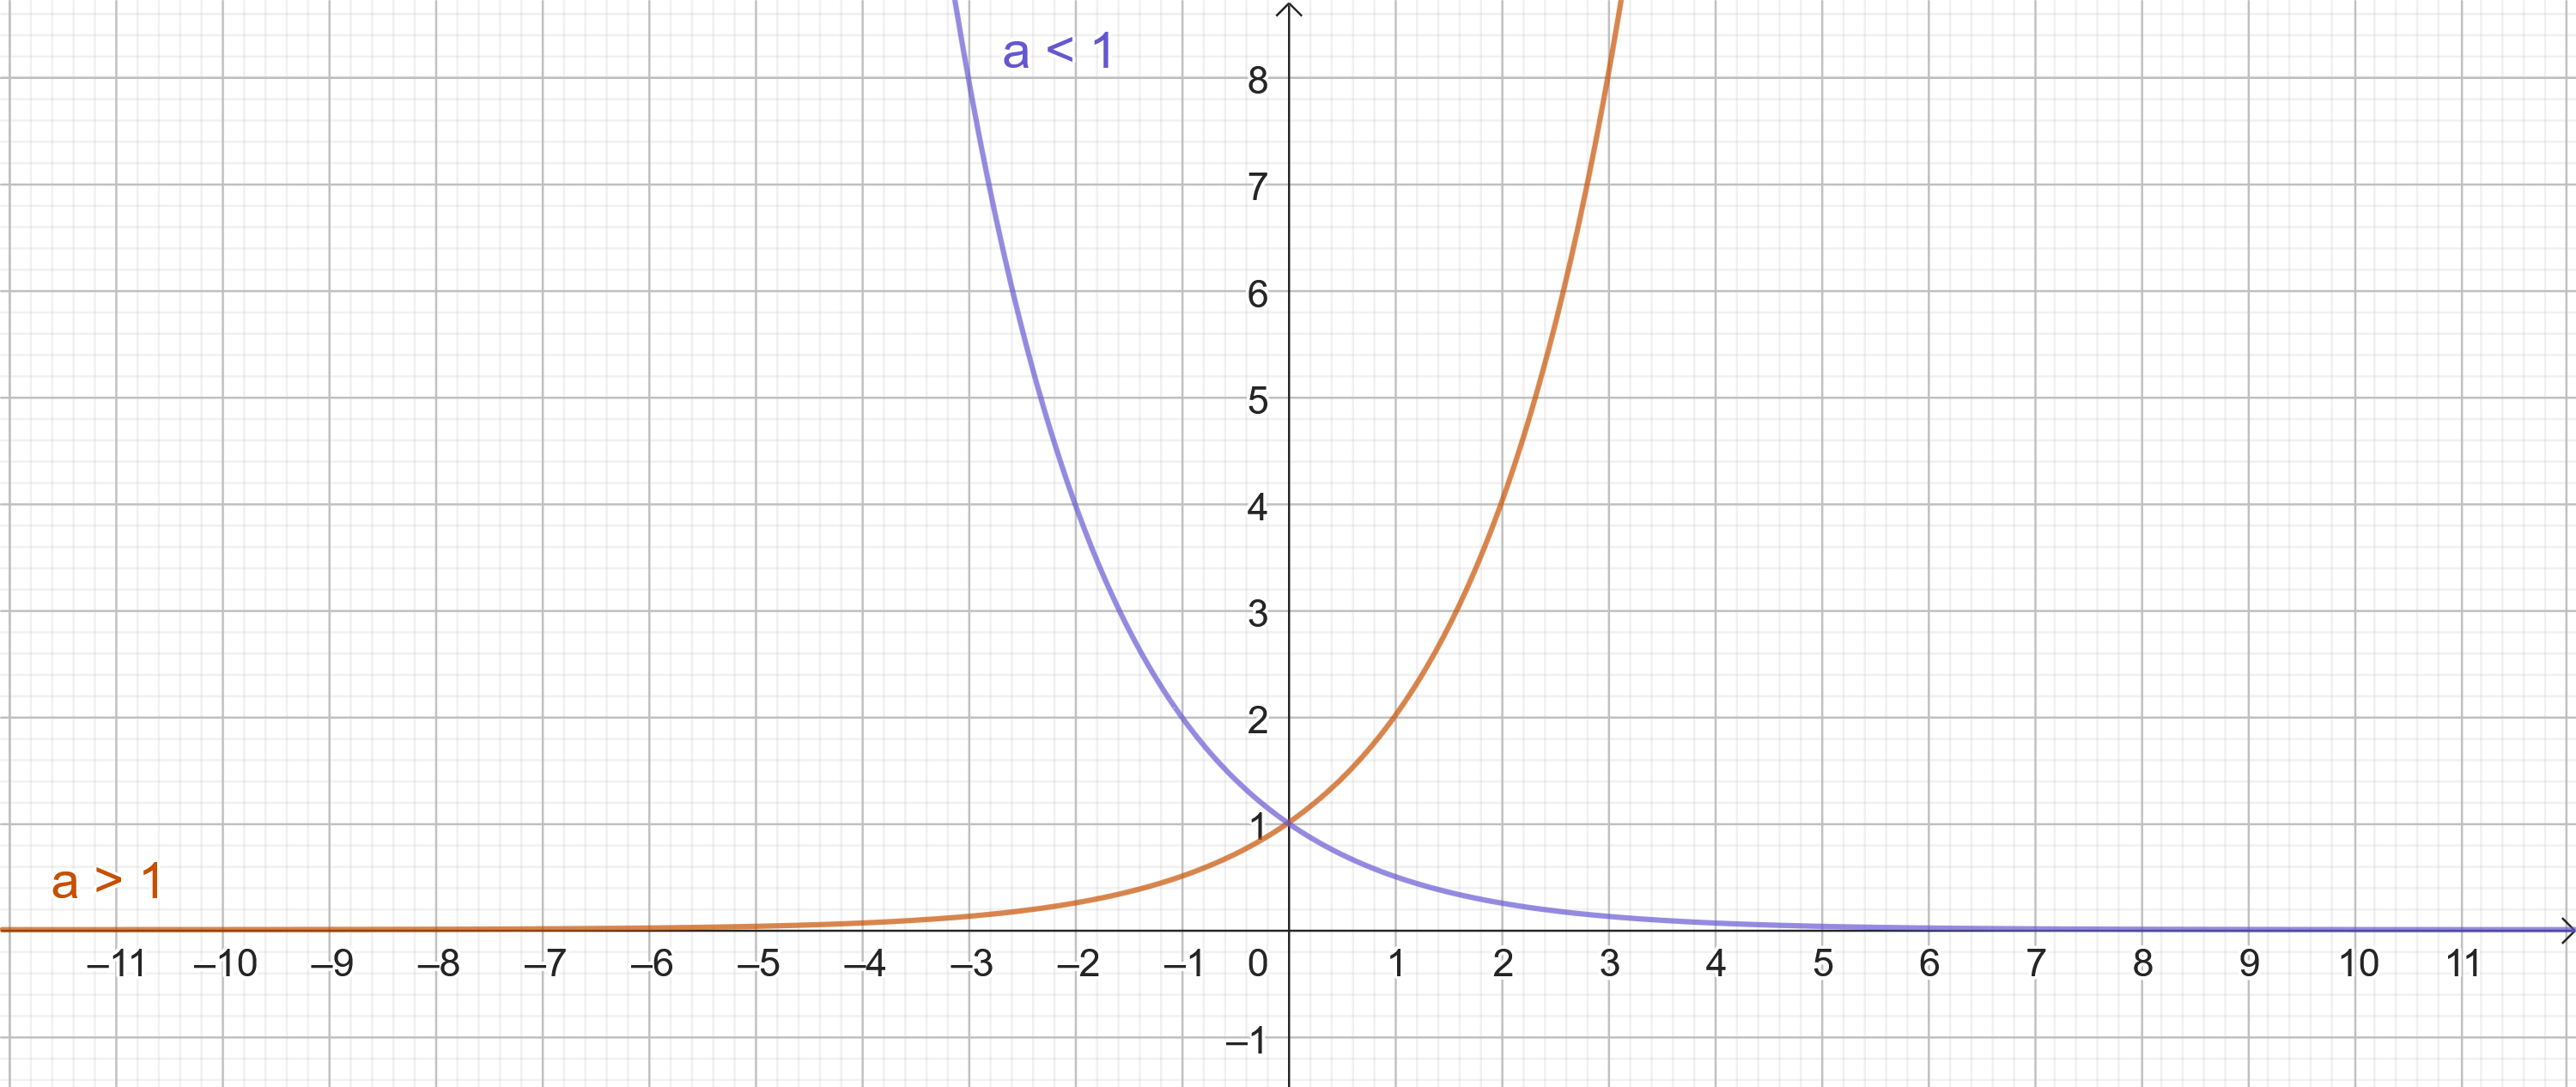
\includegraphics[width=\textwidth]{Variation_exponentielle.png}
\end{center}
\begin{example}
\hfill
\begin{enumquestions}
\item Comparer $3,4^{12}$ et $3,4^{15}$ : \answersline
\item Comparer $0,7^{3}$ et $0,7^{9}$ : \answersline
\end{enumquestions}
\end{example}
\begin{tcolorbox}
\begin{proposition}
Soit une fonction de la forme $f : x \mapsto k a^x$ avec $k$ un nombre réel et $a > 0$, alors le sens de variation de $f$ est donné grâce au tableau suivant.
\begin{center}
\begin{tabular}{|c|c|c|}
\hline
&$a > 1$&$a < 1$\\
\hline
$k > 0$& Croissante & Décroissante\\
\hline
$k < 0$& Décroissante & Croissante\\
\hline
\end{tabular}
\end{center}
\end{proposition}
\end{tcolorbox}
\end{document}